%Mettere al suo interno una suddivisione con i 4 periodi che corrispondono alle scadenze. Per ognuno suddividere ulteriormente in periodi di analisi da definire. Alla fine di ognuno dei 4 periodi principali(delle 4 scadenze) fare un Gantt
%per ogni attività bisogna trovare un sottoperiodo e per ognuno un grafico di Gantt
\section{Pianificazione} 
Il nostro gruppo, per rispettare le scadenze elencate nella sezione \textit{Calendario delle attività}, ha deciso di suddividere lo sviluppo del prodotto\glosp e della sua documentazione nelle seguenti quattro attività:
\begin{itemize}
	\item analisi dei requisiti;
	\item progettazione\glosp architetturale;
	\item progettazione\glosp di dettaglio e codifica;
	\item validazione\glosp e collaudo.
\end{itemize}
La pianificazione ha lo scopo di gestire lo sviluppo del progetto\glosp suddividendolo in attività che, singolarmente, risultano più facili da realizzare. Per descrivere ogni attività, abbiamo deciso di suddividerle ulteriormente in periodi e abbiamo elencato i ruoli attivi durante lo svolgimento di ciascuno di essi.

\subsection{Analisi dei requisiti}
L'analisi dei requisiti è il primo macro periodo: inizia il 2019-11-14, giorno successivo alla formazione dei gruppi e termina il 2020-01-20, giorno precedente alla presentazione del progetto\glo. In questa attività ci siamo principalmente interessati all'analisi di tutte le informazioni riguardanti il prodotto\glosp che dobbiamo sviluppare, l'organizzazione delle attività e la suddivisione delle risorse.

\subsubsection{Ruoli attivi}
\begin{itemize}
	\item Responsabile di progetto\glo;
	\item amministratore di progetto\glo;
	\item analista;
	\item progettista;
	\item verificatore.
\end{itemize}

\subsubsection{Periodi}
Abbiamo suddiviso il macro periodo della Analisi dei Requisiti nei seguenti sei periodi:
\paragraph*{I periodo: dal 2019-11-14 al 2019-11-27}
\begin{itemize}
	\item \textbf{Discussione dei capitolati}\glo: discussione interna, analizzando i fattori positivi e negativi di ogni capitolato\glo, per indirizzarci alla scelta di quale progetto\glosp realizzare;
	\item \textbf{Normazione}: discussione interna in merito alle regole da seguire per lo sviluppo della documentazione del progetto\glo. Iniziato il documento interno \textit{Norme di Progetto} nelle sue sezioni riguardanti: \textit{Studio di Fattibilità}, strumenti da utilizzare, documentazione, gestione della configurazione, processo\glosp di verifica e processi\glosp organizzativi;
	\item \textbf{Ricerca di strumenti e tecnologie}: inizio della ricerca di gruppo e individuale su strumenti e tecnologie necessari allo sviluppo della documentazione del progetto\glo;
	\item \textbf{Definizione dei ruoli}: suddivisione dei ruoli per le attività prese in considerazione; 
	\item \textbf{Pianificazione delle attività}: gestione delle risorse disponibili, suddivisione e pianificazione di tutte le attività che devono essere svolte in questo periodo;
	\item \textbf{Verifica}: attività di controllo dei documenti realizzati durante questo periodo.
\end{itemize}

\paragraph*{II periodo: dal 2019-11-28 al 2019-12-08}
\begin{itemize}
	\item \textbf{Studio di Fattibilità}: formalizzazione della scelta del capitolato\glosp con la stesura del documento \textit{Studio di Fattibilità v. 1.1.1};
	\item \textbf{Normazione}: revisione e aggiornamento delle \textit{Norme di Progetto} riguardanti \textit{Studio di Fattibilità} e strumenti da utilizzare;
	\item \textbf{Ricerca di strumenti e tecnologie}: continuazione della ricerca di strumenti e tecnologie da utilizzare per lo sviluppo del prodotto\glo;
	\item \textbf{Definizione dei ruoli}: suddivisione dei ruoli per le attività prese in considerazione; 
	\item \textbf{Pianificazione delle attività}: gestione delle risorse disponibili, suddivisione e pianificazione di tutte le attività che devono essere svolte in questo periodo;
	\item \textbf{Verifica}: attività di controllo dei documenti realizzati durante questo periodo.
\end{itemize}

\paragraph*{III periodo: dal 2019-12-09 al 2020-12-22}
\begin{itemize}
	\item \textbf{Normazione}: revisione e aggiornamento delle \textit{Norme di Progetto} riguardanti \textit{Analisi dei Requisiti}, \textit{Piano di Progetto} e strumenti da utilizzare;
	\item \textbf{Ricerca di strumenti e tecnologie}: continuazione della ricerca di strumenti e tecnologie da utilizzare per lo sviluppo del prodotto\glo;
	\item \textbf{Pianificazione delle attività}: gestione delle risorse disponibili, suddivisione e pianificazione di tutte le attività che devono essere svolte in questo periodo;
	\item \textbf{Analisi dei requisiti}: individuazione dei requisiti del prodotto\glosp in seguito a: incontri interni, analisi dei casi d'uso\glo, analisi del capitolato\glosp e incontro esterno col proponente.
	\item \textbf{Verifica}: attività di controllo dei documenti realizzati durante questo periodo.
\end{itemize}

\paragraph*{IV periodo: dal 2019-12-23 al 2020-01-01}
\begin{itemize}
	\item \textbf{Normazione}: revisione e aggiornamento delle \textit{Norme di Progetto} riguardanti \textit{Analisi dei Requisiti}, \textit{Piano di Qualifica}, gestione della qualità e strumenti da utilizzare;
	\item \textbf{Gestione della qualità}: inizio della discussione interna in merito a come definire e mantenere uno standard per garantire la qualità di tutti i documenti realizzati;
	\item \textbf{Ricerca di strumenti e tecnologie}: continuazione della ricerca di strumenti e tecnologie da utilizzare per lo sviluppo del prodotto\glo;
	\item \textbf{Pianificazione delle attività}: gestione delle risorse disponibili, suddivisione e pianificazione di tutte le attività che devono essere svolte in questo periodo;
	\item \textbf{Definizione dei casi d'uso}: realizzazione dei casi d'uso\glosp del prodotto\glosp richiesto dal proponente;
	\item \textbf{Verifica}: attività di controllo dei documenti realizzati durante questo periodo.
\end{itemize}


\paragraph*{V periodo: dal 2020-01-02 al 2020-01-14}
\begin{itemize}
	\item \textbf{Normazione}: revisione e aggiornamento delle \textit{Norme di Progetto} riguardanti: \textit{Piano di Qualifica}, \textit{Piano di Progetto} e strumenti da utilizzare;
	\item \textbf{Gestione della qualità}: individuazione di regole e metodi per mantenere e garantire la qualità del prodotto\glo;
	\item \textbf{Ricerca di strumenti e tecnologie}: continuazione della ricerca di strumenti e tecnologie da utilizzare per lo sviluppo del prodotto\glo;
	\item \textbf{Pianificazione delle attività}: gestione delle risorse disponibili, suddivisione e pianificazione di tutte le attività che devono essere svolte in questo periodo;
	\item \textbf{Analisi dei rischi}: discussione interna dei possibili rischi nella realizzazione del progetto\glo;
	\item \textbf{Stesura lettera di presentazione}: stesura della \textit{Lettera di Presentazione} in cui si propone una soluzione alla richiesta del proponente;
	\item \textbf{Verifica}: attività di controllo dei documenti realizzati durante questo periodo.
\end{itemize}

\paragraph*{VI periodo: dal 2020-01-15 al 2020-01-20}
\begin{itemize}
	\item \textbf{Preparazione alla discussione}: realizzazione della presentazione e preparazione individuale e di gruppo alla discussione.
\end{itemize}

\begin{figure}
	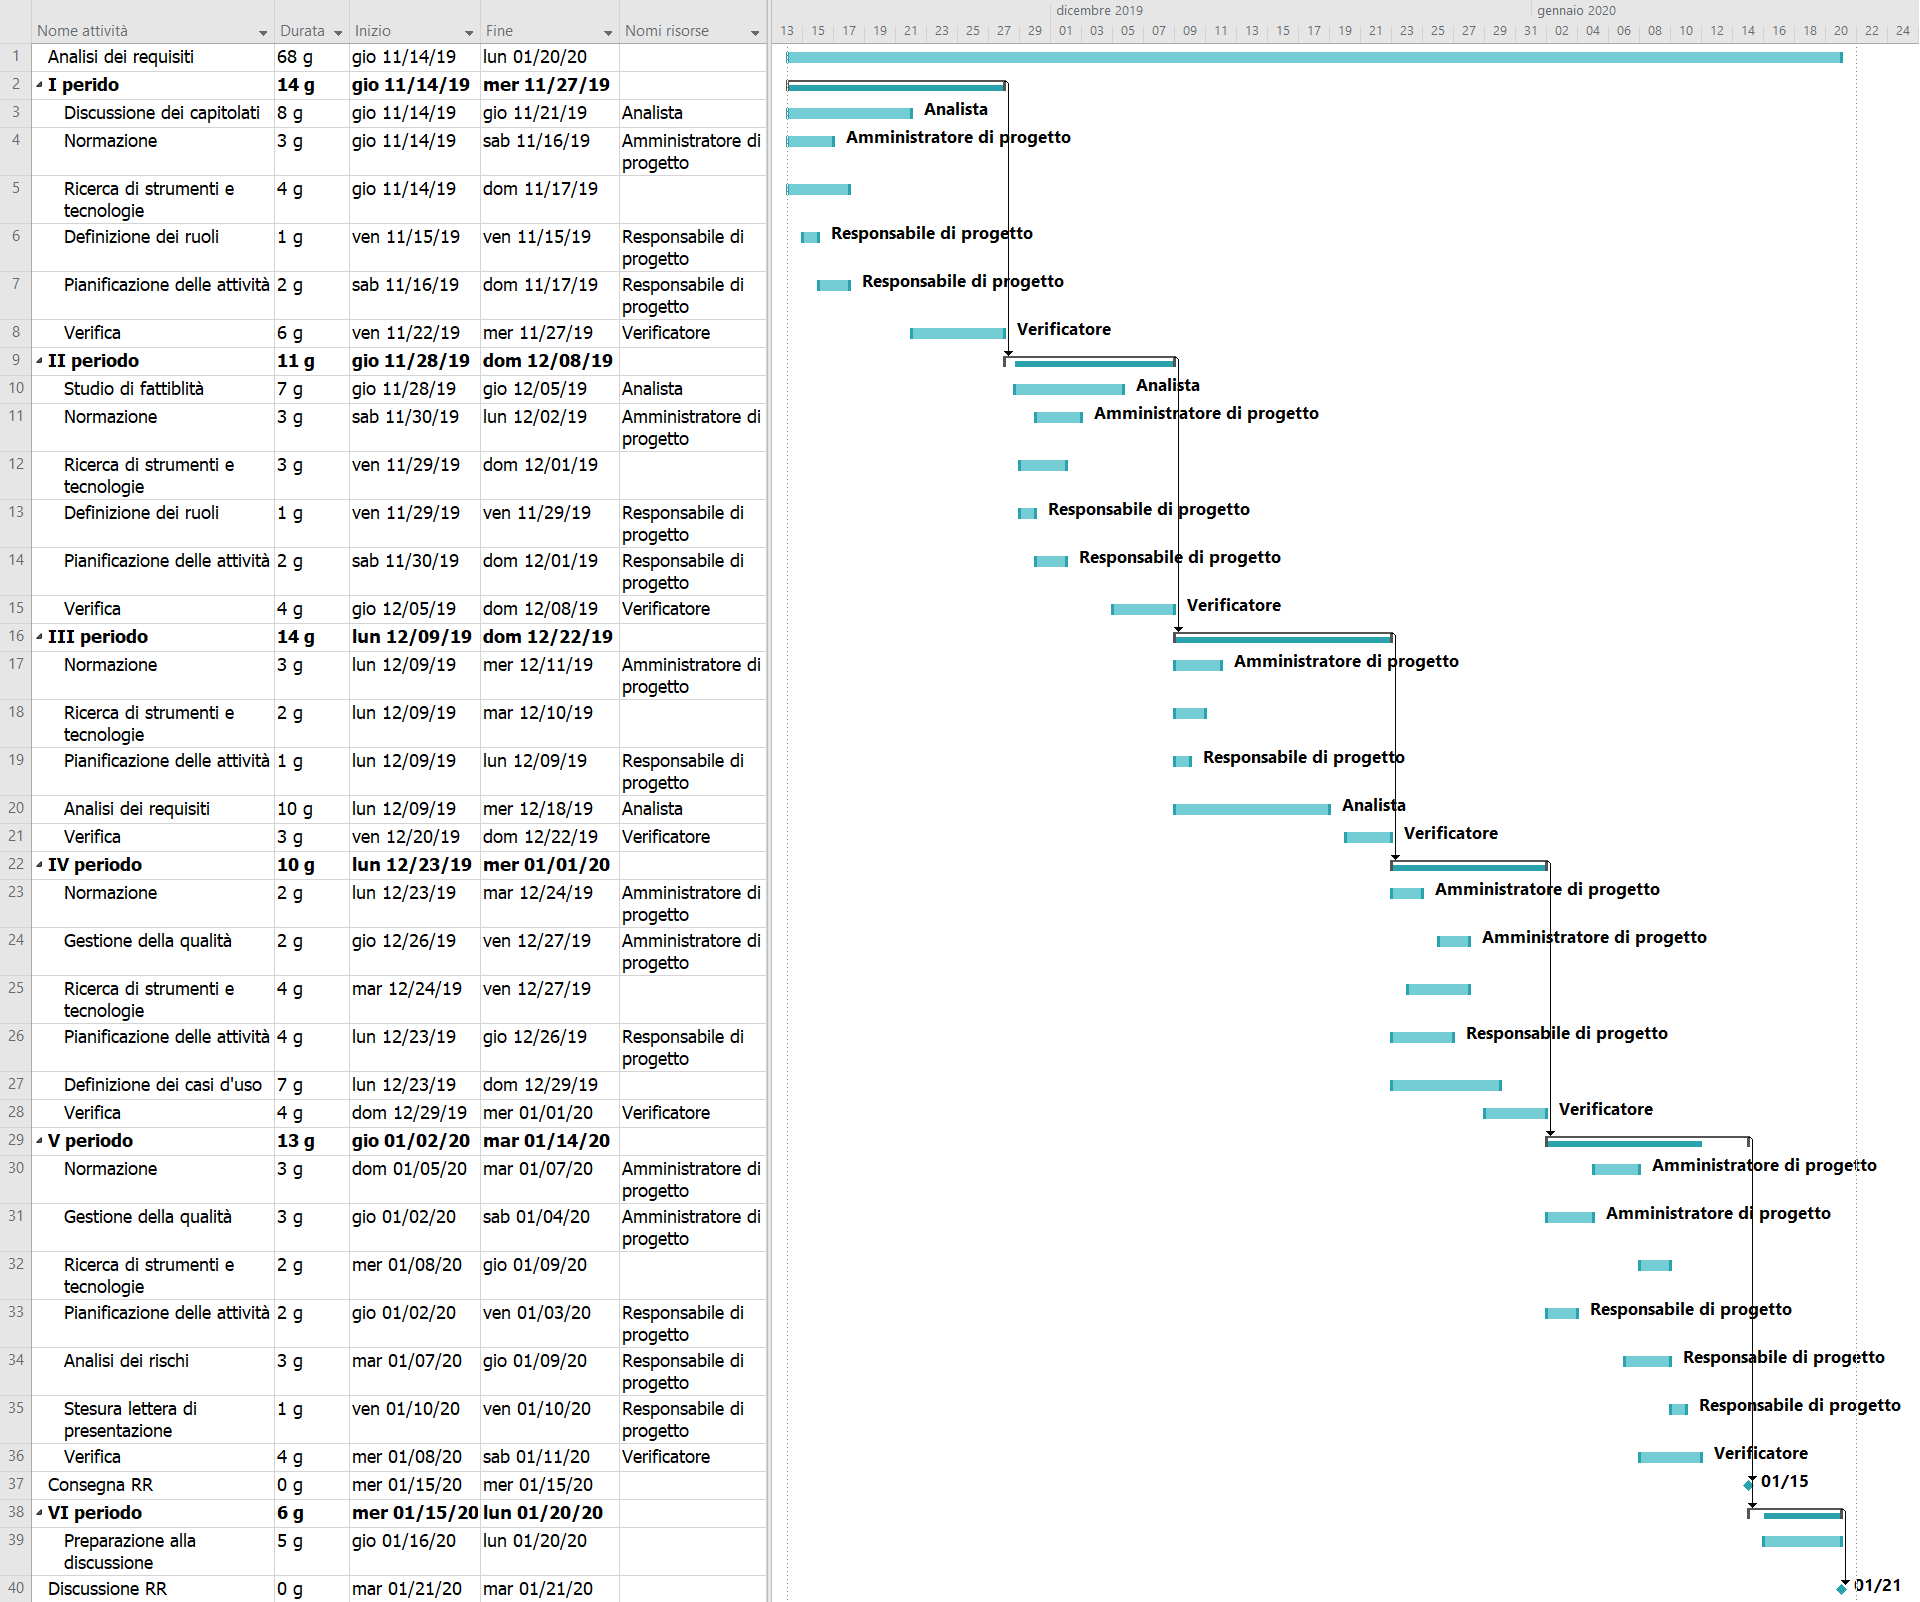
\includegraphics[width=\linewidth]{./gantt/Analisi dei requisiti.png}
	\caption{Diagramma di Gantt del periodo Analisi dei Requisiti}
\end{figure}

\subsection{Progettazione architetturale}
La progettazione\glosp architetturale è il secondo macro periodo: inizia il 2020-01-22, giorno successivo alla prima revisione e finisce il 2020-02-20, giorno precedente alla seconda revisione. In questa attività ci siamo occupati della progettazione\glosp della codifica del codice del prodotto\glo.

\subsubsection{Ruoli attivi}
\begin{itemize}
	\item Responsabile di progetto\glo;
	\item amministratore di progetto\glo;
	\item analista;
	\item progettista;
	\item programmatore;
	\item verificatore.
\end{itemize}

\subsubsection{Periodi}
\paragraph*{I periodo: dal 2020-01-22 al 2020-02-09}
\begin{itemize}
	\item \textbf{Pianificazione delle attività}: gestione delle risorse disponibili, suddivisione e pianificazione di tutte le attività che devono essere svolte in questo periodo;
	\item \textbf{Normazione}: revisione e, se necessario, aggiornamento delle \textit{Norme di Progetto};
	\item \textbf{Gestione della qualità}: revisione delle metodologie per mantenere e garantire la qualità del prodotto\glo;
	\item \textbf{Revisione dei requisiti}: revisione ed, eventualmente, modifica dei requisiti analizzati durante la prima attività in seguito a modifiche di casi d'uso\glosp o di altre indicazioni;
	\item \textbf{Ricerca di strumenti e tecnologie}: ricerca delle tecnologie necessarie allo sviluppo del progetto\glo;
	\item \textbf{Verifica}: attività di controllo dei documenti modificati durante questo periodo.
\end{itemize}

\paragraph*{II periodo: dal 2020-02-10 al 2020-02-18}
\begin{itemize}
	\item \textbf{Pianificazione delle attività}: gestione delle risorse disponibili, suddivisione e pianificazione di tutte le attività che devono essere svolte in questo periodo;
	\item \textbf{Normazione}: revisione e aggiornamento delle \textit{Norme di Progetto};
	\item \textbf{Gestione della qualità}: revisione delle metodologie per mantenere e garantire la qualità del prodotto\glo;
	\item \textbf{Configurazione di strumenti e tecnologie}: configurazione delle tecnologie necessarie allo sviluppo del progetto\glo;
	\item \textbf{Revisione dei casi d'uso}\glo: revisione e modifica dei casi d'uso\glosp in seguito a indicazioni da parte del proponente;
	\item \textbf{Revisione dei requisiti}: revisione e modifica dei requisiti analizzati durante la prima attività in seguito a modifiche di casi d'uso\glosp o di altre indicazioni;
	\item \textbf{Progettazione}\glosp\textbf{proof of concept}\glo: pianificazione dello sviluppo di una proof of concept\glosp per dimostrare la fattibilità del prodotto\glo;
	\item \textbf{Verifica}: attività di controllo dei documenti modificati durante questo periodo.
\end{itemize}

\paragraph*{III periodo: dal 2020-02-19 al 2020-02-21}
\begin{itemize}
	\item \textbf{Normazione}: revisione e aggiornamento delle \textit{Norme di Progetto};
	\item \textbf{Pianificazione delle attività}: gestione delle risorse disponibili, suddivisione e pianificazione di tutte le attività che devono essere svolte in questo periodo;
	\item \textbf{Codifica proof of concept}\glo: sviluppo del codice per realizzare il proof of concept\glosp precedentemente pianificato, implementazione degli incrementi 1 e 9 del modello di sviluppo incrementale;
	\item \textbf{Stesura lettera di presentazione}: stesura della \textit{Lettera di Presentazione} in cui si propone una soluzione alla richiesta del proponente;
	\item \textbf{Verifica}: attività di controllo dei documenti e del codice sorgente realizzati durante questo periodo.
\end{itemize}

\paragraph*{IV periodo: dal 2020-02-22 al 2020-02-25}
\begin{itemize}
	\item \textbf{Pianificazione delle attività}: gestione delle risorse disponibili, suddivisione e pianificazione di tutte le attività che devono essere svolte in questo periodo;
	% Verificare se scrivere incremento 7 e 15 come parziali: nel PoC faremo solo esportazione del file e visualizzazione dei dati
	% Da incremento 7 eventualmente togliere "creazione"
	% Da incremento 15 eventualmente togliere "elaborazione"
	\item \textbf{Codifica proof of concept}\glo: sviluppo del codice per realizzare il proof of concept\glosp precedentemente pianificato, implementazione degli incrementi 2, 7, 12 e 15 del modello di sviluppo incrementale;
	\item \textbf{Verifica}: attività di controllo dei documenti e del codice sorgente realizzati durante questo periodo.
\end{itemize}

\paragraph*{V periodo: dal 2020-02-26 al 2020-03-08}
\begin{itemize}
	\item \textbf{Studio di strumenti e tecnologie}: revisione delle tecnologie e degli strumenti necessari per lo sviluppo del prodotto\glosp richiesto dal proponente in seguito alla presentazione dei PoC\glosp agli stakeholder\glo;
	\item \textbf{Normazione}: revisione e aggiornamento delle \textit{Norme di Progetto};
	\item \textbf{Pianificazione delle attività}: gestione delle risorse disponibili, suddivisione e pianificazione di tutte le attività che devono essere svolte in questo periodo;
	\item \textbf{Progettazione}\glosp\textbf{proof of concept}\glo: eventuale revisione della progettazione\glosp della proof of concept\glosp per dimostrare la fattibilità del prodotto\glo;
	\item \textbf{Codifica proof of concept}\glo: aggiornamento del codice del proof of concept\glosp in seguito alla presentazione agli stakeholder\glo;
	\item \textbf{Stesura lettera di presentazione}: stesura della \textit{Lettera di Presentazione} in cui si propone una soluzione alla richiesta del proponente;
	\item \textbf{Verifica}: attività di controllo dei documenti e del codice sorgente realizzati durante questo periodo.
\end{itemize}

\paragraph*{VI periodo: dal 2020-03-09 al 2020-03-15}
\begin{itemize}
	\item \textbf{Preparazione alla discussione}: realizzazione della presentazione e preparazione individuale e di gruppo alla discussione.
\end{itemize}

\begin{landscape}
	\begin{figure}
		\centering
		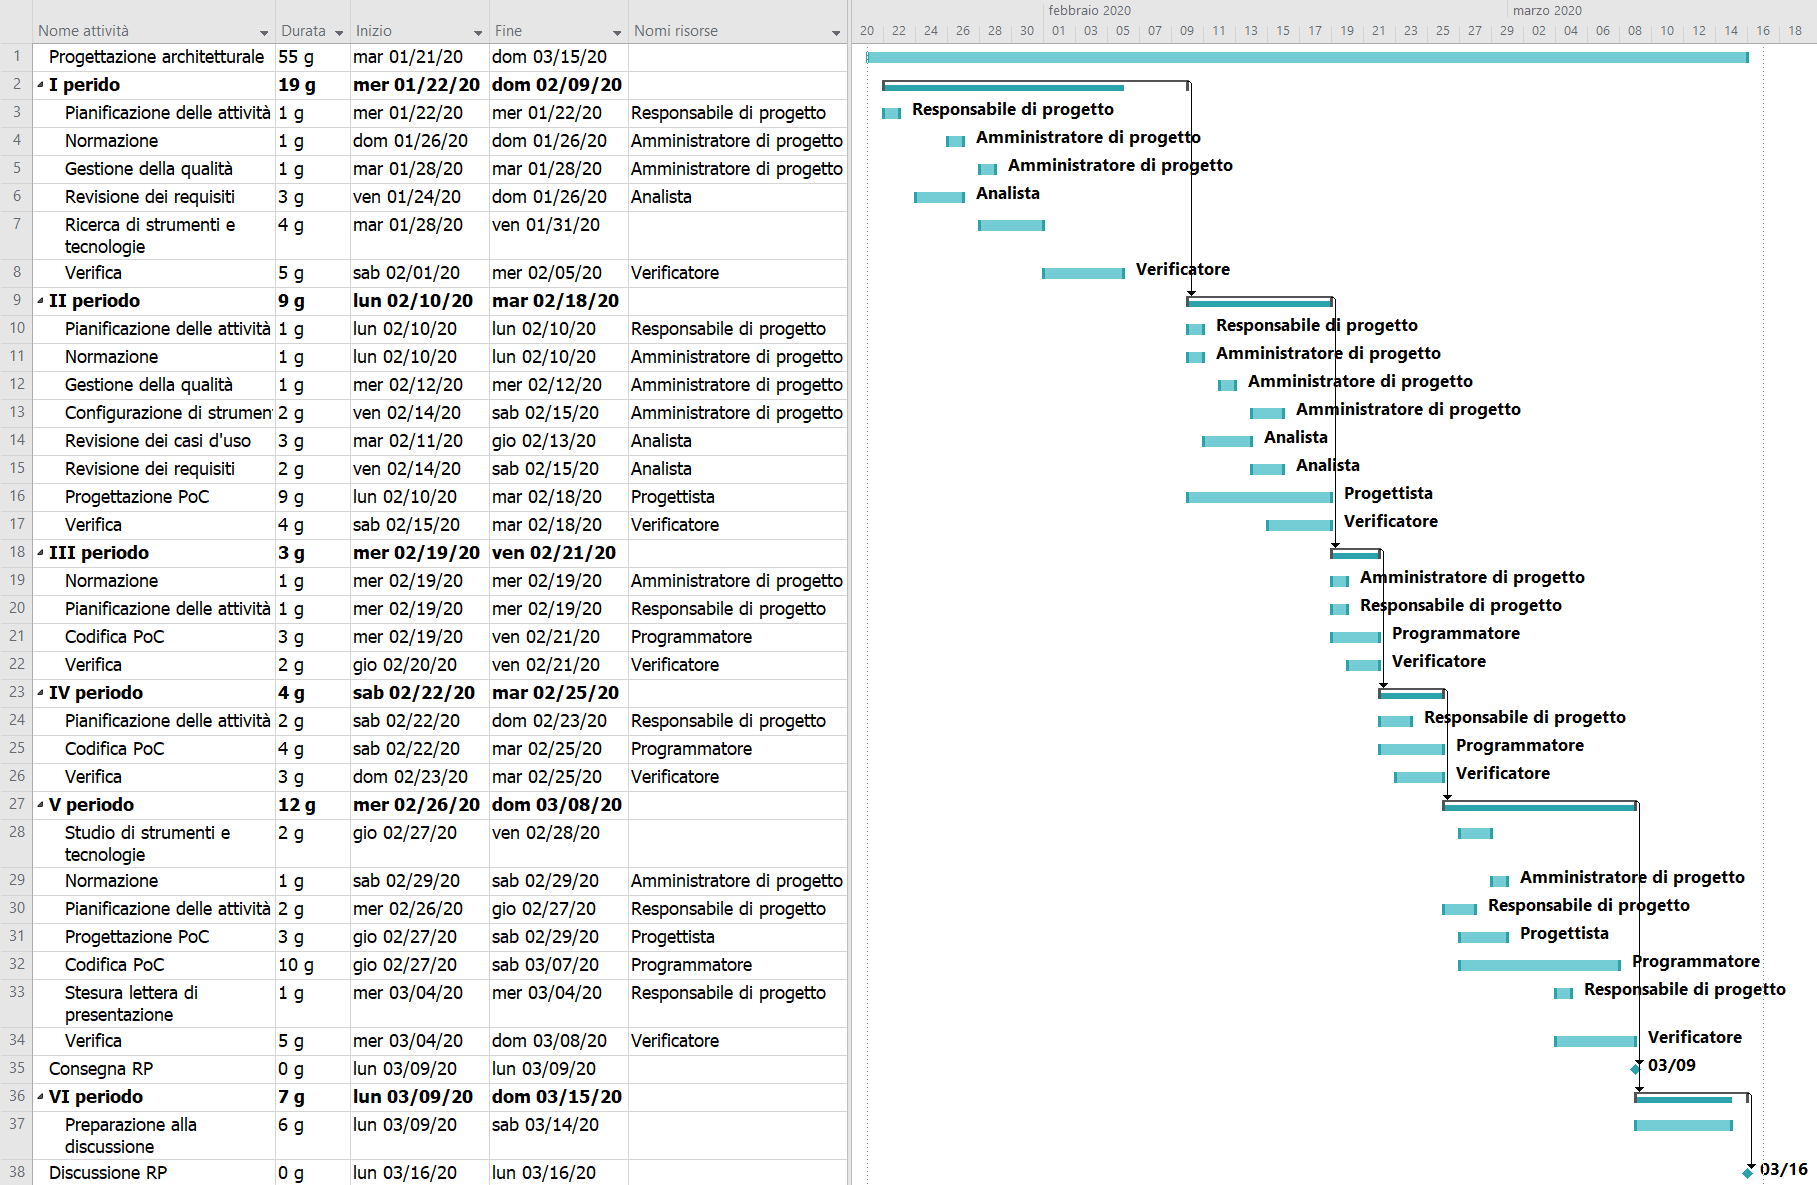
\includegraphics[scale=0.512]{./gantt/Progettazione architetturale.png}
		\caption{Diagramma di Gantt del periodo Progettazione Architetturale}
	\end{figure}
\end{landscape}


\subsection{Progettazione di dettaglio e codifica}
La progettazione\glosp di dettaglio e codifica è il nostro terzo macro periodo: inizia il 2020-03-17, giorno successivo alla seconda revisione e finisce il 2020-04-19, giorno precedente alla terza revisione. Durante lo svolgimento di questa attività ci occuperemo principalmente della codifica del codice del prodotto\glo.

\subsubsection{Ruoli attivi}
\begin{itemize}
	\item Responsabile di progetto\glo;
	\item amministratore di progetto\glo;
	\item analista
	\item progettista;
	\item programmatore;
	\item verificatore.
\end{itemize}

\subsubsection{Incrementi e periodi}
Durante la progettazione\glosp di dettaglio e codifica, pianifichiamo di sviluppare i seguenti incrementi:
\begin {itemize}
	\item incremento 3;
	\item incremento 4;
	\item incremento 6;
	\item incremento 13;
	\item incremento 14;
	\item incremento 16.
\end {itemize}
Di seguito analizziamo la pianificazione di dettaglio per quanto concerne lo sviluppo di ciascun incremento.
\paragraph{Incremento 3} \mbox{} \\ \\ 
L'incremento 3 prevede lo sviluppo e l'implementazione dell'algoritmo di addestramento SVM\glosp nell'applicazione esterna e nel plug-in. 
\\Prevede il soddisfacimento completo o parziale dei seguenti requisiti:
\begin{itemize}
	\item R1F4.2;
	\item R1F4.10;
	\item R1F11.
\end{itemize}
Viene svolto in un unico periodo.
\mbox{} \\ \\ \textbf{I periodo: dal 2020-03-17 al 2020-03-24} \mbox{} \\ \\
\textbf{Ruoli attivi}
\begin{itemize}
	\item Responsabile di progetto\glo;
	\item amministratore di progetto\glo;
	\item analista
	\item progettista;
	\item programmatore;
	\item verificatore.
\end{itemize}
\textbf{Attività} 
\begin{itemize}
	\item \textbf{Revisione dei documenti}: revisione e, se necessario, aggiornamento dei documenti secondo le indicazioni del committente;
	\item \textbf{Normazione}: revisione e, se necessario, aggiornamento delle \textit{Norme di Progetto};
	\item \textbf{Ricerca di strumenti e tecnologie}: ricerca e studio degli strumenti e tecnologie utilizzate per la codifica;
	\item \textbf{Pianificazione delle attività}: gestione delle risorse disponibili, suddivisione e pianificazione di tutte le attività che devono essere svolte in questo periodo;
	\item \textbf{Progettazione}\glo: definizione in modo più dettagliato ed eventuali correzioni dell'architettura del nostro prodotto\glosp software con rispettiva individuazione dei design pattern architetturali da applicare e progettazione\glosp dell'incremento 3; 
	\item \textbf{Revisione dei requisiti}: revisione ed, eventualmente, modifica dei requisiti analizzati secondo le indicazioni; 
	\item \textbf{Codifica}: scrittura del codice del prodotto\glosp seguendo le indicazioni definite nel documento \textit{Norme di Progetto} e nella progettazione\glosp indicata sopra. Codifica per l'implementazione dell'incremento 3; 
	\item \textbf{Verifica}: attività di controllo dei documenti e del codice realizzati durante questo periodo.
\end{itemize}
\paragraph{Incremento 4} \mbox{} \\ \\
L'incremento 4 prevede lo sviluppo e l'implementazione dell'algoritmo di addestramento RL\glosp nell'applicazione esterna e nel plug-in.
\\Prevede il soddisfacimento completo o parziale dei seguenti requisiti:
\begin{itemize}
	\item R1F4.11; 
\end{itemize}
Viene svolto in un unico periodo.
\mbox{} \\ \\ \textbf{II periodo: dal 2020-03-25 al 2020-03-30} \mbox{} \\ \\
\textbf{Ruoli attivi}
\begin{itemize}
	\item Responsabile di progetto\glo;
	\item amministratore di progetto\glo;
	\item analista
	\item progettista;
	\item programmatore;
	\item verificatore.
\end{itemize}
\textbf{Attività} 
\begin{itemize}
	\item \textbf{Normazione}: revisione e, se necessario, aggiornamento delle \textit{Norme di Progetto};
	\item \textbf{Ricerca di strumenti e tecnologie}: ricerca e studio degli strumenti e tecnologie utilizzate per la codifica;
	\item \textbf{Pianificazione delle attività}: gestione delle risorse disponibili, suddivisione e pianificazione di tutte le attività che devono essere svolte in questo periodo;
	\item \textbf{Progettazione}\glo: revisione e aggiornamento della progettazione\glosp dell'architettura del prodotto\glosp con rispettiva individuazione dei design pattern architetturali da applicare e progettazione\glosp dell'incremento 4; 
	\item \textbf{Revisione dei requisiti}: revisione ed, eventualmente, modifica dei requisiti analizzati secondo le indicazioni; 
	\item \textbf{Codifica}: scrittura del codice del prodotto\glosp seguendo le indicazioni definite nel documento \textit{Norme di Progetto} e nella progettazione\glosp indicata sopra. Codifica per l'implementazione dell'incremento 4;
	\item \textbf{Scrittura manuale sviluppatore}: inizio della scrittura del \textit{Manuale dello sviluppatore} per fornire le indicazioni utili ad uno sviluppatore che vuole contribuire al progetto\glo; 
	\item \textbf{Verifica}: attività di controllo dei documenti e del codice realizzati durante questo periodo.
\end{itemize}
\paragraph{Incremento 6} \mbox{} \\ \\
L'incremento 6 prevede lo sviluppo e l'implementazione della funzionalità che permette all'utente di selezionare un modello di predizione e avviare l'addestramento dello stesso.
\\Prevede il soddisfacimento completo o parziale dei seguenti requisiti:
\begin{itemize}
	\item R1F4.11;
	\item R1F4.12;
	\item R1F4.4.
\end{itemize}
Viene svolto in un unico periodo.
\mbox{} \\ \\ \textbf{III periodo: dal 2020-03-31 al 2020-04-02} \mbox{} \\ \\
\textbf{Ruoli attivi}
\begin{itemize}
	\item Responsabile di progetto\glo;
	\item amministratore di progetto\glo;
	\item progettista;
	\item programmatore;
	\item verificatore.
\end{itemize}
\textbf{Attività} 
\begin{itemize}
	\item \textbf{Normazione}: revisione e, se necessario, aggiornamento delle \textit{Norme di Progetto};
	\item \textbf{Ricerca di strumenti e tecnologie}: ricerca e studio degli strumenti e tecnologie utilizzate per la codifica;
	\item \textbf{Pianificazione delle attività}: gestione delle risorse disponibili, suddivisione e pianificazione di tutte le attività che devono essere svolte in questo periodo;
	\item \textbf{Progettazione}\glo: progettazione\glosp dell'incremento 6;  
	\item \textbf{Codifica}: scrittura del codice del prodotto\glosp seguendo le indicazioni definite nel documento \textit{Norme di Progetto} e nella progettazione\glosp indicata sopra. Codifica per l'implementazione dell'incremento 6;
	\item \textbf{Scrittura manuale sviluppatore}: aggiornamento del \textit{Manuale dello sviluppatore};
	\item \textbf{Verifica}: attività di controllo dei documenti e del codice realizzati durante questo periodo.
\end{itemize}
\paragraph{Incremento 13} \mbox{} \\ \\
L'incremento 13 prevede lo sviluppo e l'implementazione della lettura del file di configurazione, che sarà in formato JSON, e la conseguente configurazione degli algoritmi.
\\Prevede il soddisfacimento completo o parziale dei seguenti requisiti:
\begin{itemize}
	\item R1F8;
	\item R1F11.
\end{itemize}
Viene svolto in un unico periodo.
\mbox{} \\ \\ \textbf{IV periodo: dal 2020-04-03 al 2020-04-05} \mbox{} \\ \\
\textbf{Ruoli attivi}
\begin{itemize}
	\item Responsabile di progetto\glo;
	\item amministratore di progetto\glo;
	\item progettista;
	\item programmatore;
	\item verificatore.
\end{itemize}
\textbf{Attività} 
\begin{itemize}
	\item \textbf{Normazione}: revisione e, se necessario, aggiornamento delle \textit{Norme di Progetto};
	\item \textbf{Pianificazione delle attività}: gestione delle risorse disponibili, suddivisione e pianificazione di tutte le attività che devono essere svolte in questo periodo;
	\item \textbf{Progettazione}\glo: progettazione\glosp dell'incremento 13;  
	\item \textbf{Codifica}: scrittura del codice del prodotto\glosp seguendo le indicazioni definite nel documento \textit{Norme di Progetto} e nella progettazione\glosp indicata sopra. Codifica per l'implementazione dell'incremento 13;
	\item \textbf{Scrittura manuale sviluppatore}: aggiornamento del \textit{Manuale dello sviluppatore};
	\item \textbf{Scrittura manuale utente}: inizio della scrittura del \textit{Manuale utente} per descrivere come deve l'utente finale deve utilizzare il software;
	\item \textbf{Verifica}: attività di controllo dei documenti e del codice realizzati durante questo periodo.
\end{itemize}
\paragraph{Incremento 14} \mbox{} \\ \\
L'incremento 14 prevede lo sviluppo e l'implementazione dell'associazione dei nodi al flusso dati e dell'elaborazione e visualizzazione dei dati.
\\Prevede il soddisfacimento completo o parziale dei seguenti requisiti:
\begin{itemize}
	\item R1F9;
	\item R1F9.1;
	\item R1F9.2;
	\item R1F9.4;
	\item R1F9.5.
\end{itemize}
Viene svolto in un unico periodo.
\mbox{} \\ \\ \textbf{V periodo: dal 2020-04-6 al 2020-04-10} \mbox{} \\ \\
\textbf{Ruoli attivi}
\begin{itemize}
	\item Responsabile di progetto\glo;
	\item amministratore di progetto\glo;
	\item progettista;
	\item programmatore;
	\item verificatore.
\end{itemize}
\textbf{Attività} 
\begin{itemize}
	\item \textbf{Normazione}: revisione e, se necessario, aggiornamento delle \textit{Norme di Progetto};
	\item \textbf{Pianificazione delle attività}: gestione delle risorse disponibili, suddivisione e pianificazione di tutte le attività che devono essere svolte in questo periodo;
	\item \textbf{Progettazione}\glo: progettazione\glosp dell'incremento 14;  
	\item \textbf{Codifica}: scrittura del codice del prodotto\glosp seguendo le indicazioni definite nel documento \textit{Norme di Progetto} e nella progettazione\glosp indicata sopra. Codifica per l'implementazione dell'incremento 14;
	\item \textbf{Scrittura manuale sviluppatore}: aggiornamento del \textit{Manuale dello sviluppatore};
	\item \textbf{Scrittura manuale utente}: aggiornamento del \textit{Manuale utente};
	\item \textbf{Verifica}: attività di controllo dei documenti e del codice realizzati durante questo periodo.
\end{itemize}
\paragraph{Incremento 16} \mbox{} \\ \\
L'incremento 16 prevede lo sviluppo e l'implementazione della funzionalità che permette all'utente di arrestare l'algoritmo di addestramento prima del suo termine naturale.
\\Prevede il soddisfacimento completo o parziale dei seguenti requisiti:
\begin{itemize}
	\item R1F12;
	\item R1F20.
\end{itemize}
Viene svolto in un unico periodo.
\mbox{} \\ \\ \textbf{VI periodo: dal 2020-04-11 al 2020-04-13} \mbox{} \\ \\
\textbf{Ruoli attivi}
\begin{itemize}
	\item Responsabile di progetto\glo;
	\item amministratore di progetto\glo;
	\item progettista;
	\item programmatore;
	\item verificatore.
\end{itemize}
\textbf{Attività} 
\begin{itemize}
	\item \textbf{Normazione}: revisione e, se necessario, aggiornamento delle \textit{Norme di Progetto};
	\item \textbf{Pianificazione delle attività}: gestione delle risorse disponibili, suddivisione e pianificazione di tutte le attività che devono essere svolte in questo periodo;
	\item \textbf{Progettazione}\glo: progettazione\glosp dell'incremento 16;  
	\item \textbf{Codifica}: scrittura del codice del prodotto\glosp seguendo le indicazioni definite nel documento \textit{Norme di Progetto} e nella progettazione\glosp indicata sopra. Codifica per l'implementazione dell'incremento 16;
	\item \textbf{Scrittura manuale sviluppatore}: chiusura del \textit{Manuale dello sviluppatore};
	\item \textbf{Scrittura manuale utente}: chiusura del \textit{Manuale utente};
	\item \textbf{Stesura lettera di presentazione}: stesura della \textit{Lettera di Presentazione} in cui si propone una soluzione alla richiesta del proponente;
	\item \textbf{Verifica}: attività di controllo dei documenti e del codice realizzati durante questo periodo.
\end{itemize}
\paragraph{VII periodo: dal 2020-04-14 al 2020-04-19}
\begin{itemize}
	\item \textbf{Preparazione alla discussione}: realizzazione della presentazione e preparazione individuale e di gruppo alla discussione.
\end{itemize}

\begin{figure}
	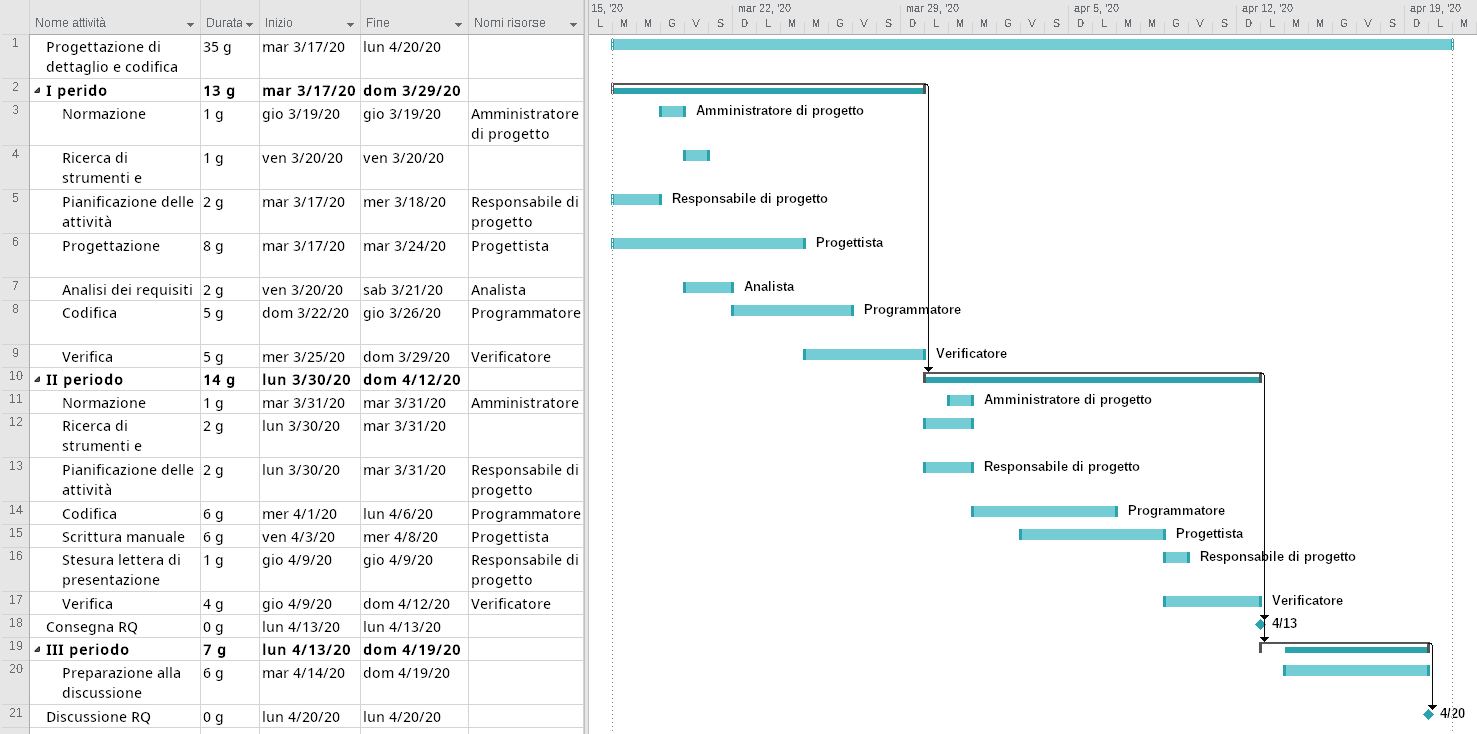
\includegraphics[width=\linewidth]{./gantt/Progettazione di dettaglio e codifica.png}
	\caption{Diagramma di Gantt del periodo Progettazione di dettaglio e codifica}
\end{figure}

\subsection{Validazione e collaudo}
Validazione\glosp e collaudo il quarto macro periodo: inizia il 2020-04-21, giorno successivo alla terza revisione e si conclude il 2020-05-17, giorno precedente all'ultima revisione. In questa attività ci occuperemo del collaudo e della validazione\glosp del prodotto\glosp per verificare che tutti i requisiti definiti come obbligatori nell'\textit{Analisi dei Requisiti} siano stati soddisfatti.

\subsubsection{Ruoli attivi}
\begin{itemize}
	\item Responsabile di progetto\glo;
	\item amministratore di progetto\glo;
	\item progettista;
	\item programmatore;
	\item verificatore.
\end{itemize}

\subsubsection{Periodi}
\paragraph*{I periodo: dal 2020-04-21 al 2020-04-30}
\begin{itemize}
	\item \textbf{Normazione}: revisione e, se necessario, aggiornamento delle \textit{Norme di Progetto};
	\item \textbf{Ricerca di strumenti e tecnologie}: ricerca e studio degli strumenti e tecnologie utilizzate per la codifica del codice;
	\item \textbf{Pianificazione delle attività}: gestione delle risorse disponibili, suddivisione e pianificazione di tutte le attività che devono essere svolte in questo periodo;
	\item \textbf{Gestione qualità}: revisione, e se necessario, le metodologie per la mantenere il livello di qualità prestabilito;
	\item \textbf{Revisione dei requisiti}: revisione e, se necessario, aggiornamento dei requisiti del progetto\glo;
	\item \textbf{Verifica}: controllo dei documenti realizzati durante questo periodo.
\end{itemize}

\paragraph*{II periodo: dal 2020-05-01 al 2020-05-10}
\begin{itemize}
	\item \textbf{Revisione manuale d'uso}: revisione e, se necessario, aggiornamento del \textit{Manuale d'Uso};
	\item \textbf{Codifica}: implementazione degli incrementi mancanti del prodotto\glosp seguendo le indicazioni delle \textit{Norme di Progetto} e della progettazione\glosp indicata sopra;
	\item \textbf{Test e collaudo}: scrittura dei test mancanti per il collaudo finale del prodotto\glo;
	\item \textbf{Stesura lettera di presentazione}: stesura della \textit{Lettera di Presentazione} che in cui si propone una soluzione alla richiesta del proponente;
	\item \textbf{Verifica}: attività di controllo del codice e dei documenti realizzati durante questo periodo.
\end{itemize}

\paragraph*{III periodo: dal 2020-05-12 al 2020-05-17}
\begin{itemize}
	\item \textbf{Preparazione alla discussione}: realizzazione della presentazione e preparazione individuale e di gruppo alla discussione.
\end{itemize}
\begin{landscape}
	\begin{figure}
		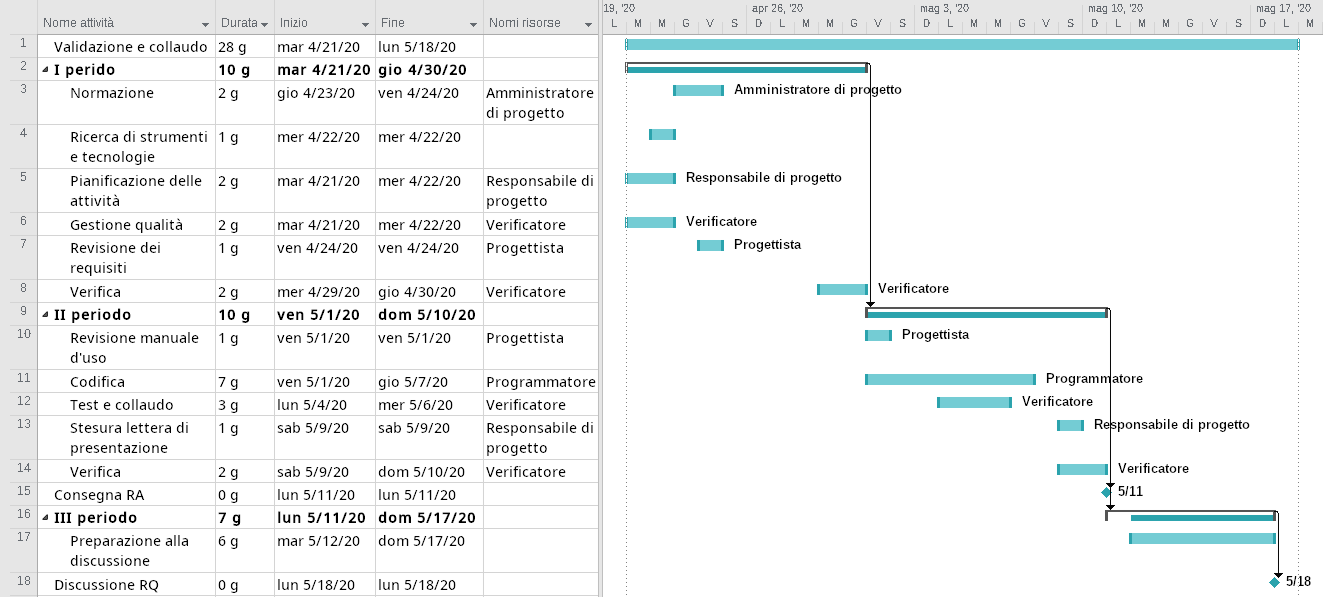
\includegraphics[width=\linewidth]{./gantt/Validazione e collaudo.png}
		\caption{Diagramma di Gantt del periodo Validazione e collaudo}
	\end{figure}
\end{landscape}
